\section{YOLO} \label{yolo}

\begin{figure}[!htbp]
    \centering
    \centerline{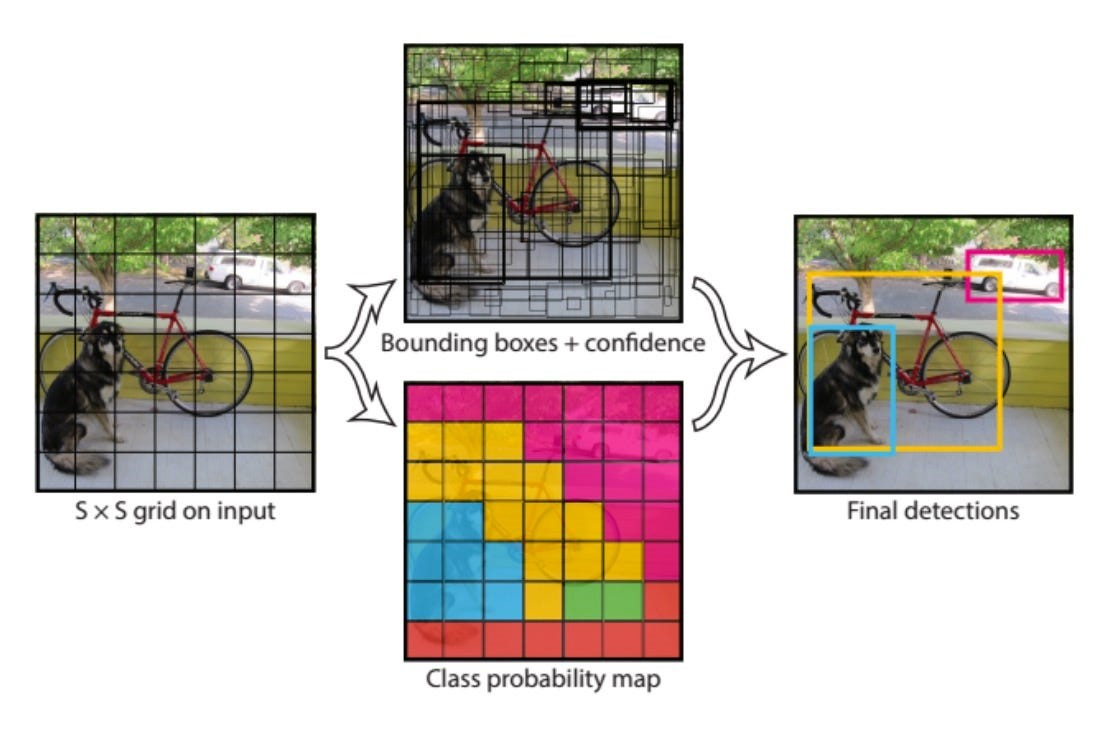
\includegraphics[width=0.8\linewidth]{images/yolo_object_detection.jpg}}
    \caption{YOLO model for object detection \cite{redmonYouOnlyLook2016}}
    \label{fig:yolo_diagram}
\end{figure}
YOLO (You Only Look Once) is a convolutional neural network (CNN) and is commonly used for object detection. As shown in figure \ref{fig:yolo_diagram}, the model divides an image into a grid of cells and predicts the bounding boxes, the confidence score of the bounding box, and the class probability for each grid cell that may contain an object in a single evaluation \cite{redmonYouOnlyLook2016}. The framework has developed from its original iteration with more improved versions under its name, such as YOLO9000 or YOLOv2 \cite{redmonYOLO9000BetterFaster2016}, YOLOv3 \cite{redmonYOLOv3IncrementalImprovement2018}, and YOLOv4 \cite{bochkovskiyYOLOv4OptimalSpeed2020}, with YOLOv8 as its latest model \cite{jocherYOLOUltralytics2023}.

\begin{table}[!htbp]
    \centering
    \caption{YOLO framework models}
    \resizebox{0.8\linewidth}{!}
    {
    \begin{tabular}{c c c}
        \hline
        YOLO Model & Training Dataset & Performance (AP)  \\
        \hline
        YOLOv1 & PASCAL VOC & {63.4\%}  \\
        \hline
        YOLOv2/YOLO9000 & PASCAL VOC & 78.6\% \\
        \hline
        YOLOv3 & MS COCO & 36.2\% \\
        \hline
        YOLOv4 & MS COCO & 43.5\% \\
        \hline
        YOLOv5 & MS COCO & 55.8\%\\
        \hline
        YOLOv6 & MS COCO & 52.5\% \\
        \hline
        YOLOv7 & MS COCO & 55.9\% \\
        \hline
        YOLOv8 & MS COCO & 53.9\% \\
        \hline
    \end{tabular}
    }
    \label{tab:yolo1-8}
\end{table}

Table \ref{tab:yolo1-8} displays the various models and their respective performance over time  \cite{tervenComprehensiveReviewYOLO2023}, and explains that the AP is lower across the latter models because of the number of object categories the MS COCO dataset contain (80) compared to the PASCAL VOC 2007 dataset (20). For the purpose of this study, the YOLOv3 model will be used due to the extensive studies done using it as shown in Table \ref{tab:yolo_studies}, as well as the ethical issues raised \cite{sagarYOLOCreatorQuits2020}.

\begin{table}[]
    \centering
    \caption{YOLO model related literatures}
    \resizebox{0.8\linewidth}{!}
    {
    \begin{tabular}{c c c}
        \hline
        YOLO Model Used & Study & Purpose  \\
        \hline
        \multirow{5}{*}{YOLOv3} &  \cite{liuApplicationYoloMask2021, sevillaMaskVisionMachineVisionBased2021} & Mask Detection \\\cline{2-3}
         & \cite{xuEfficientPedestrianDetection2022, rakhsithFaceMaskSocial2021, srinivasanCOVID19MonitoringSystem2021, gongPedestrianDetectionAlgorithm2022} & Pedestrian Detection \\\cline{2-3}
         & \cite{chakarDepthwiseSeparableConvolutions2020, ghoshDeepNetworkPruning2019} & Model Size Reduction \\\cline{2-3}
         & \cite{liYOLOv3LiteLightweightCrack2019} & Fault Detection \\\cline{2-3}
         & \cite{sunYoloBasedLightweightObject2023} & Lightweight Deployment \\
        \hline
        \multirow{2}{*}{YOLOv3-tiny} & \cite{liFireObjectDetection2022} & Fire Detection \\\cline{2-3}
        & \cite{qianEfficientModelCompression2018} & Model Size Reduction \\
        \hline
        \multirow{2}{*}{YOLOv4} & \cite{bhambaniRealtimeFaceMask2020} & Pedestrian Detection \\\cline{2-3}
        & \cite{sarmientoPavementDistressDetection2021} & Fault Detection \\
        \hline
        YOLOv4-tiny & \cite{sathyamurthyRealtimeFaceMask2021, liberatoriYOLOBasedFaceMask2022} & Mask Detection \\
        \hline
        YOLOv5 & \cite{youssryAccurateRealTimeFace2022} & Mask Detection \\
        \hline
    \end{tabular}
    }
    \label{tab:yolo_studies}
\end{table}
